\documentclass[a4paper, 12pt]{article}
\usepackage[utf8]{inputenc}
\usepackage[spanish]{babel}
\usepackage{url, hyperref}
\usepackage{graphicx}
\usepackage{listings, xcolor}

\definecolor{codegreen}{rgb}{0,0.6,0}
\definecolor{codegray}{rgb}{0.5,0.5,0.5}
\definecolor{codepurple}{rgb}{0.58,0,0.82}
\definecolor{backcolour}{rgb}{0.95,0.95,0.92}
\lstdefinestyle{mystyle}{
    backgroundcolor=\color{backcolour},   
    commentstyle=\color{codegreen},
    keywordstyle=\color{magenta},
    numberstyle=\tiny\color{codegray},
    stringstyle=\color{codepurple},
    basicstyle=\ttfamily\footnotesize,
    breakatwhitespace=false,         
    breaklines=true,                 
    captionpos=b,                    
    keepspaces=true,                 
    numbers=left,                    
    numbersep=5pt,                  
    showspaces=false,                
    showstringspaces=false,
    showtabs=false,                  
    tabsize=2
}

\setlength{\parindent}{0pt}
\lstset{style=mystyle}

\title{
    \vspace{-3cm}Tarea 2: Investigación de lenguajes de programación
    para robots
    \author{
        Universidad Autónoma de San Luis Potosí\\
        Facultad de Ingeniería - Ing. En Sistemas Inteligentes\\
        \textbf{Materia:} Programación de Robots\\
        \textbf{Prof:} Dr. César Augusto Puente Montejano\\
        \textbf{Autor:} Angel de Jesús Maldonado Juárez
    }
    \date{\textbf{Fecha de entrega:} viernes 3 de febrero de 2023}
}

\begin{document}
\maketitle

\hrule

\section*{\emph{V+}}
La empresa \emph{SimPhonics} se dedica al desarrollo y venta de
sistemas de audio de alta fidelidad, y en el año 1993 tras la salida
de la nueva tarjeta FX-3000 las placas de programación utilizaban este
estándar para las nuevas tecnologías, por lo que los sistemas de la
empresa tuvieron que evolucionar también, y de esta manera se inició
el desarrollo del entorno y lenguaje visual de programación \emph{V+}
en los principios de los 90s.

Algunas de las características del lenguaje son que simplifica el
proceso de desarrollo/programación debido a que se manejan bloques
visuales en lugar de texto, el paradigma de \emph{V+} está pensado para
que los programadores implementen soluciones para una gran variedad de
sistemas de hardware (audio, motores, computadoras, robots, etc.)o
software como simuladores.

Un programa visual en \emph{V+}, \emph{llamado diseño}, se compone de
\textbf{objetos} y \textbf{puertos}, conectados por redes que se
distribuyen en la hoja de trabajo. Un diseño típico en \emph{V+} consiste
en una o más hojas de trabajo. Ejemplo de un diseño en \emph{V+}:

\begin{figure}[!ht]
    \centering
    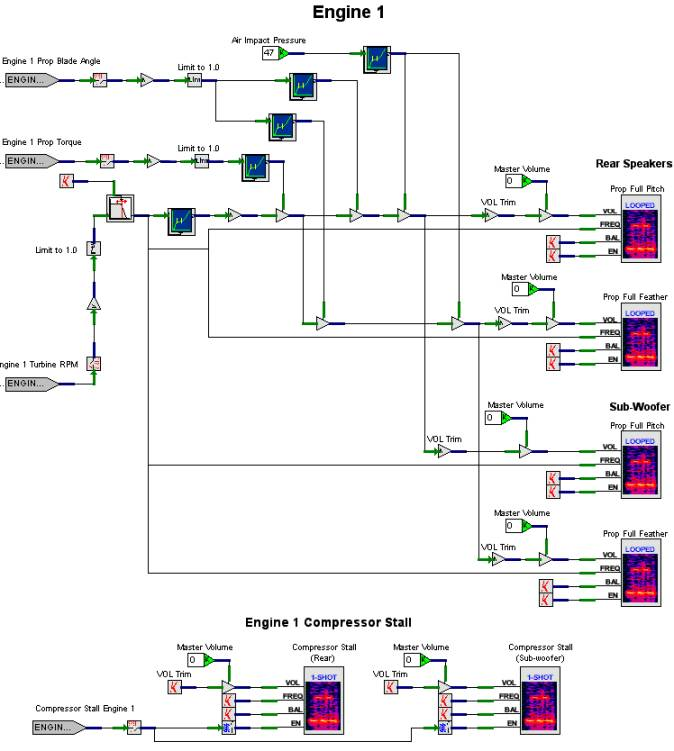
\includegraphics[width=0.25\textwidth]{img/vp_sample.jpg}
    \caption{Imagen original}
\end{figure}

\section*{\emph{AML}}
\emph{A Manufacturing Language} (\emph{AML}) fue creado por \emph{IBM} durante
las decadas de los 70s y 80s, principalmente para su robot \emph{RS1}. Algunas
de las extensiones de \emph{AML} son \emph{AML/2}, \emph{AML/E}, \emph{AML/V},
y \emph{AML/X}, además, todos los programas en \emph{AML} pueden utilizar
subrutinas escritas en \emph{C} o \emph{FORTRAN}, el paradigma del lenguaje es
el paradigma imperativo (procedural). El rango de aplicaciones de \emph{AML}
va desde acceder a opciones y funcionalidades de bajo nivel en el hardware, hasta
crear aplicaciones con interfaces gráficas (\emph{GUI}), pero es utilizado
ampliamente en el campo de la robótica.
El siguiente código es un ejemplo de un programa escrito en \emph{AML}, llamado
\emph{peg-in-hole}.

\lstinputlisting{src/aml_sample.aml}

\section*{\emph{VAL}}
\emph{Variable Assembly Language} (\emph{VAL}) es todo un sistema computarizado
y un lenguaje de programación que fue diseñado para la \emph{Unimation Inc.},
la primera empresa de robótica del mundo, desarrollado en 1973 en la
\emph{Universidad de Stanford}. El lenguaje de programación de robots
\emph{VAL} permite la ejecución de movimientos complejos de manera rápida y
eficiente, también tiene un buen manejo de la memoria del sistema por lo que es
posible la ejecución en tiempo-real, y es posible considerar la interacción
humana de forma simultánea a la automatización del robot.
El siguiente código es un ejemplo de programa escrito en \emph{VAL}:

\lstinputlisting{src/val_sample.val}

\section*{\emph{Webots}}
\emph{Webots} es un software multi-plataforma y opensource utilizado para
simular robots, este provee todo un ambiente para modelar, programar, y simular
todo tipo de robots. Fue diseñado y pensado para un uso profesional, y actualmente
es bastante utilizado en la industria, educación, e investigación. \emph{Webots} fue
creado y es mantenido actualmente por \emph{Cyberbotics Ltd} desde 1998.
Las características principales de \emph{Webots} es que utiliza la librería \emph{Qt}
para realizar la interfaz gráfica del programa, junto con su propia versión del
motor de físicas \emph{ODE}, además del motor de gráficos \emph{wren} con \emph{OpenGL},
lo cual permite que el software pueda ser utilizado en \emph{Windows}, \emph{Linux}, y
\emph{MacOS}.

Uno de los robots más representativos en los cuales se utiliza \emph{Webots} para
realizar las simulaciones es \emph{Dexter}, el cual consiste en dos brazos con
manipuladores para realizar laparoscopias.

\begin{figure}[!ht]
    \centering
    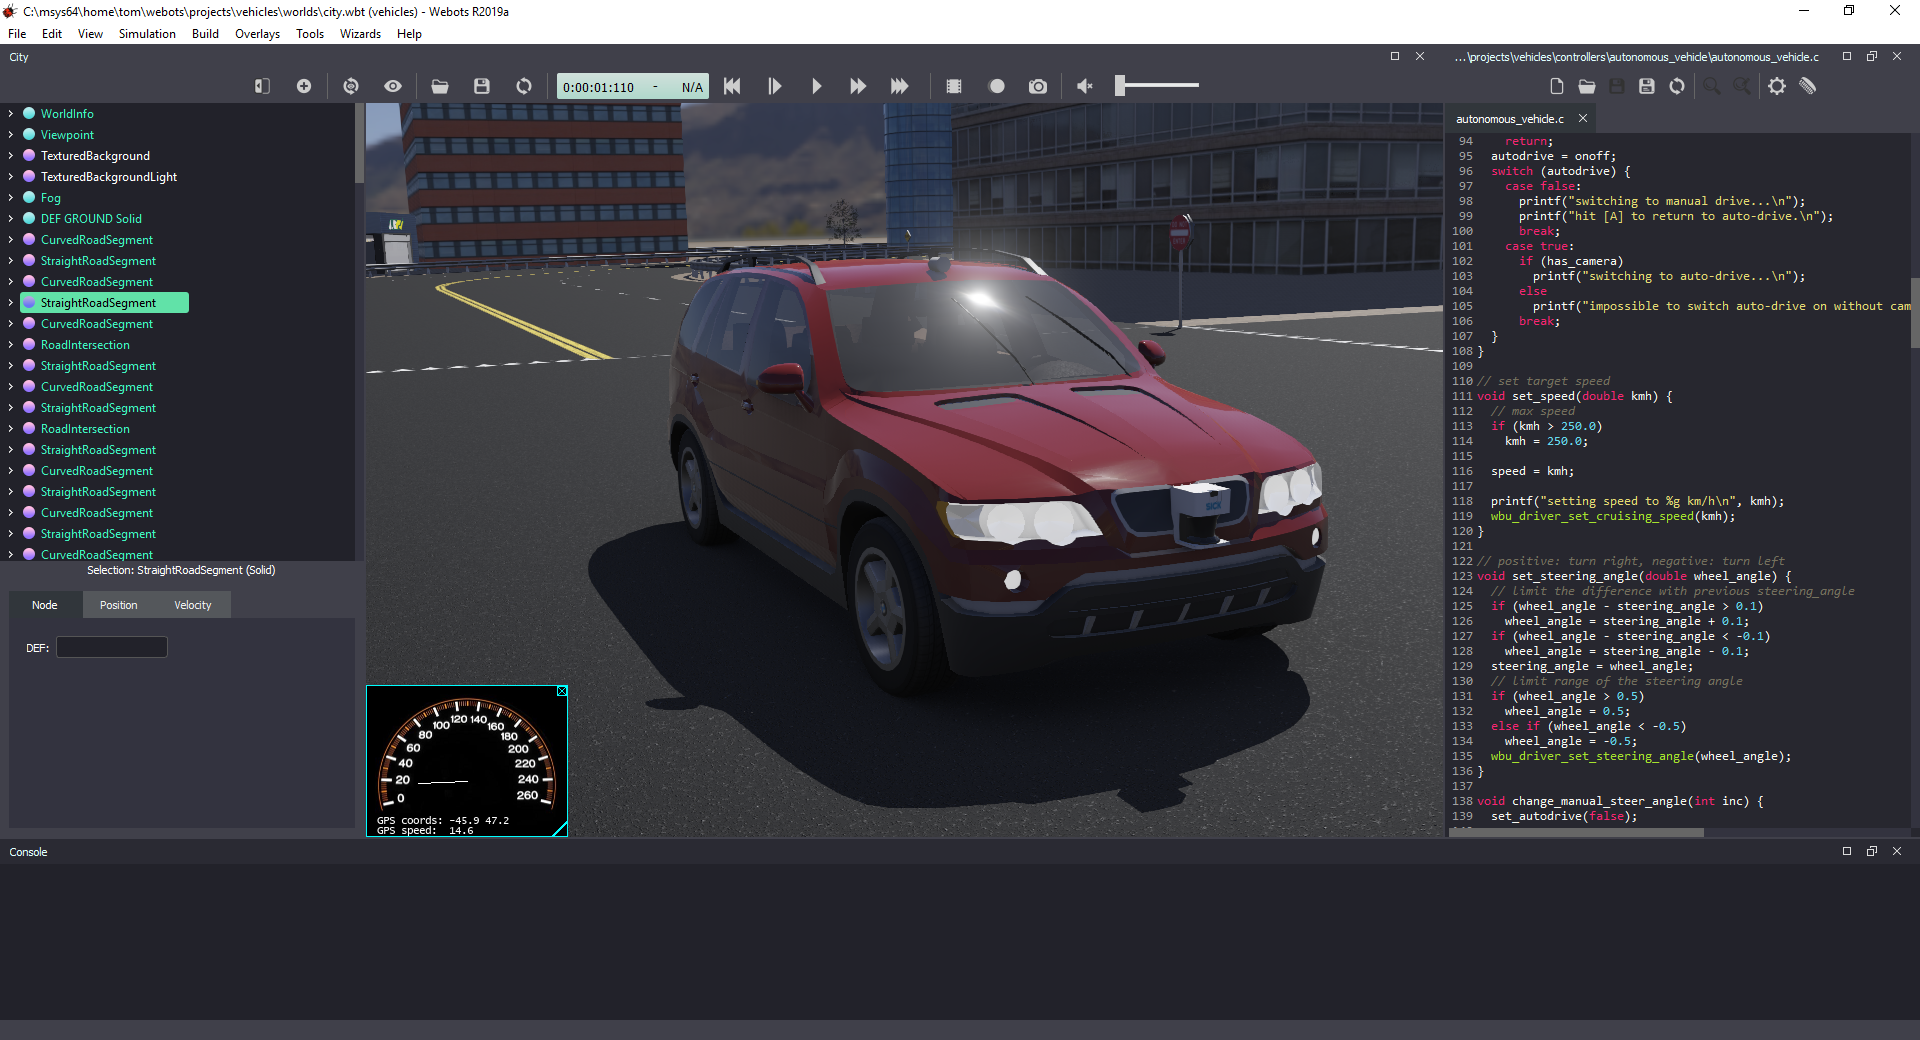
\includegraphics[width=0.8\textwidth]{img/Wbinterface.png}
    \caption{Interfaz de \emph{Webots}}
\end{figure}

\hrule

\bibliographystyle{plain}
\bibliography{refs}
\nocite{*}
\end{document}